\documentclass[12pt, titlepage]{article}
\usepackage[margin=1in]{geometry}
\usepackage{graphicx}
\graphicspath{ {./survey_results/} }
\usepackage[dvipsnames]{xcolor}
\usepackage{booktabs}
\usepackage{changepage}
\usepackage{tabularx}
\usepackage{longtable}
\usepackage{hyperref}
\usepackage{multirow}
\usepackage{array}
\usepackage{float}
\usepackage{mdframed}
\usepackage{amssymb}
\usepackage{setspace}
\usepackage{amsmath}
\usepackage{tikz}
\hypersetup{
    colorlinks,
    citecolor=black,
    filecolor=black,
    linkcolor=red,
    urlcolor=blue
}
\usepackage[round]{natbib}
%% Comments

\usepackage{color}

\newif\ifcomments\commentstrue %displays comments
%\newif\ifcomments\commentsfalse %so that comments do not display

\ifcomments
\newcommand{\authornote}[3]{\textcolor{#1}{[#3 ---#2]}}
\newcommand{\todo}[1]{\textcolor{red}{[TODO: #1]}}
\else
\newcommand{\authornote}[3]{}
\newcommand{\todo}[1]{}
\fi

\newcommand{\wss}[1]{\authornote{blue}{SS}{#1}} 
\newcommand{\plt}[1]{\authornote{magenta}{TPLT}{#1}} %For explanation of the template
\newcommand{\an}[1]{\authornote{cyan}{Author}{#1}}

%% Common Parts

\newcommand{\progname}{Sayyara Automotive Matcher} % PUT YOUR PROGRAM NAME HERE
\newcommand{\authname}{Team 27, Kappastone
\\ Tevis Doe, doet
\\ Caitlin Bridel, bridelc
\\ Gilbert Cherrie, cherrieg
\\ Rachel Johnson, johnsr12
\\ Harkeerat Kanwal, kanwalh
\\ Himanshu Aggarwal, aggarwah} % AUTHOR NAMES                  

\usepackage{hyperref}
    \hypersetup{colorlinks=true, linkcolor=blue, citecolor=blue, filecolor=blue,
                urlcolor=blue, unicode=false}
    \urlstyle{same}
                                


\begin{document}

\title{Verification and Validation Report: \progname} 
\author{\authname}
\date{\today}
	
\maketitle

\pagenumbering{roman}

\section{Revision History}

\begin{tabularx}{\textwidth}{p{3cm}p{2cm}X}
\toprule {\bf Date} & {\bf Version} & {\bf Notes}\\
\midrule
8 March 2023 & 1.0 & First iteration of V\&V Report \\
Date 2 & 1.1 & Notes\\
\bottomrule
\end{tabularx}

~\newpage

\section{Symbols, Abbreviations and Acronyms}

\renewcommand{\arraystretch}{1.2}
\begin{tabular}{l l} 
  \toprule		
  \textbf{symbol} & \textbf{description}\\
  \midrule 
  T & Test\\
  FT-RT & Functional Requirement Test \\
  NFT-LF & Non-Functional Look and Feel Requirement Test \\
  NFT-UT & Non-Functional Usability Requirement Test \\
  \bottomrule
\end{tabular}\\

\wss{symbols, abbreviations or acronyms -- you can reference the SRS tables if needed}

\newpage

\tableofcontents

\listoftables %if appropriate

\listoffigures %if appropriate

\newpage

\pagenumbering{arabic}

This document covers the results of the actions carried out detailed in the Verification and Validation Plan.

\section{Functional Requirements Evaluation}

%\begin{table}[H]
%\centering
The following table summarizes the results of the functional tests provided in our \href{https://github.com/HKanwal/kapstone/blob/main/docs/VnVPlan/VnVPlan.pdf}{Verification and Validation Plan}.
\renewcommand{\arraystretch}{1.8}%
\begin{longtable}{| m{.1\linewidth} |>{\raggedright\arraybackslash} m{.15\linewidth} |>{\raggedright\arraybackslash} m{.22\linewidth}|>{\raggedright\arraybackslash} m{.21\linewidth} |>{\raggedright\arraybackslash} m{.21\linewidth}|>{\centering\arraybackslash} m{.08\linewidth}|}
\caption{Functional Test Description and Results}
\label{tab:funcTestResults}
\\ \hline
\textbf{Test ID} & \textbf{Description} & \textbf{Inputs} & \textbf{Expected Output} & \textbf{Actual Output} & \textbf{Result} \\
\hline
\endfirsthead

\multicolumn{6}{c}
{{\bfseries \tablename\ \thetable{} -- continued from previous page}} \\
\hline \multicolumn{1}{|c|}{\textbf{Test ID}} & \multicolumn{1}{c|}{\textbf{Description}} & \multicolumn{1}{c|}{\textbf{Inputs}} & \multicolumn{1}{c|}{\textbf{Expected Output}} & \multicolumn{1}{c|}{\textbf{Actual Output}} & \multicolumn{1}{c|}{\textbf{Result}} \\ \hline 
\endhead

\hline \multicolumn{6}{|r|}{{Continued on next page}} \\ \hline
\endfoot

\endlastfoot
FT-RT-1 & Create a shop on a newly created shop owner account & Randomly generated shop name, hours of Monday 10:00 to 17:00, 2 bays, an address of 123 Main Rd., Hamilton, Ontario, Canada, A1B2C3 and then save is clicked. & A shop is created in the database with these values and added to the shop profile for the currently signed in shop owner account and the user is redirected to the dashboard. & A shop is created in the database with these values and added to the shop profile for the currently signed in shop owner account and the user is redirected to the dashboard. & \textcolor{Green}{Pass} \\
\hline
FT-RT-2 & Navigate to the registration page and create a shop owner account. & Navigate to registration page, and enter values of First Name: John, Last Name: Smith, Phone Number: +16472224448, email: test@email.com, a randomly generated username, Password: ShopPass123, and select Shop Owner from the account type drop down. Then click the Create button. & A shop owner account is created with the provided values and the user in redirected to the Create Shop Page & A shop owner account is created with the provided values and the user in redirected to the Create Shop Page & \textcolor{Green}{Pass}\\
\hline
FT-RT-3 & Employees should receive invitation email when they are invited & Cypress is used to navigate to the invitations page and enter the employee's email. After a short wait, it queries the Email API server to check if the invitation email was received by the employee. & The employee has received an email with a link to register an account. & The email was successfully sent to the employee with a valid invitation link. &  \textcolor{Green}{Pass}\\
\hline
FT-RT-4 & Employees should be able to use the invitation link in their invite email to register for an employee account. & Cypress is used to fetch the link in the employee's email. The link is visited and details are their details are entered. & The page should navigate to the dashboard. & The page successfully navigated to the dashboard page.  & \textcolor{Green}{Pass}\\
\hline
FT-RT-5 & Navigate to employee profile/ details page and edit employee information & Log in to shop owner account, navigate to employee list page, click on random employee from the list. Click pencil icon to enter edit mode and change Salary value to a different randomized value and click Save button  & Employee information is updated with new inputted information & Employee information is updated with new inputted information & \textcolor{Green}{Pass}\\
\hline
FT-RT-5.1 & Navigate to shop owner profile/ details page and edit shop owner information & Log in to shop owner account, navigate to employee list page, click on shop owner from the list. Click pencil icon to enter edit mode and change account information and click Save button  & Shop owner information is updated with new inputted information & Unable to find shop owner in list & \textcolor{Red}{Fail}\\
\hline
FT-RT-6 & Employee account should be deleted and removed from shop on request. & Cypress is used to login to an employee account, visit the account page, and click on the 'Delete Account' button. & The employee's account is deleted from the database and should be removed from the shop's employee list. & No option present to delete the employee. & \textcolor{Red}{Fail}\\
\hline
FT-RT-7 & Shop owners should be able to add, remove, and search for employees. & Cypress is used to login as a shop owner and navigate to the employee pages (invite page, list view, detail view) to verify if these features work successfully. & The shop owner is able to access all of the employee pages, filter them using search and add/delete them. & The shop owner was able to access all of the employee pages, filter them using search and add/delete them & \textcolor{Green}{Pass}\\
\hline
FT-RT-7.1 & Employees and customers should not be able to access pages related to employee management. & Cypress is used to login as a employee/customer and navigate to the employee pages (invite page, list view, detail view). & The pages should automatically redirect to the 404 page. & The pages automatically redirected to the 404 page. & \textcolor{Green}{Pass}\\
\hline
FT-RT-8 & Test whether a previously created shop owner, employee and customer account and able to login. & Navigate to the login page and enter valid credentials for a shop owner account and click login. Then repeat this test with an employee account and customer account credentials. & For all the account types the user is able to login and is redirected to the dashboard after successfully logging in. & For all account types the user is able to login and redirected to the dashboard after successfully logging in. & \textcolor{Green}{Pass}\\
\hline
FT-RT-9 & User with customer account can create a quote request and submit it to a list of shops and then view the details & Login to customer account, navigate to quote request page and enter the following details: VIN = '123456789', manufacturer = 'BMW', model = 'i7', modelYear = '2005', shop = "Sam's Workshop", quoteRequest = `QUOTEREQUEST-[random integer]` and click Create button. Navigate to quote request list page, find card containing quote request name, click on the card and confirm detail page opens and all details match inputted information.  & Quote request is submitted, can be viewed by customer and details match inputted information & Quote request is submitted, can be viewed by customer and details match inputted information & \textcolor{Green}{Pass}\\
\hline
FT-RT-9.1 & User with shop owner account can view the details of a quote request sent to their shop & Log in to customer account, navigate to quote request page and enter the following details: VIN = '123456789', manufacturer = 'BMW', model = 'i7', modelYear = '2005', shop = "Sam's Workshop", quoteRequest = `QUOTEREQUEST-[random integer]` and click Create button. Log in to shop owner account, navigate to new quote request list page, find card containing quote request name, click on the card and confirm detail page opens and all details match inputted information.  & Quote request is submitted to shop owner's shop, can be viewed by shop owner and details match inputted information & Quote request is submitted to shop owner's shop, can be viewed by shop owner and details match inputted information & \textcolor{Green}{Pass}\\
\hline
FT-RT-10 & Shop owner can respond to quote request sent to their shop and then view the details of the quote & Create quote request on customer account. Login to shop owner account, navigate to new quote request list page and click card containing quote request name. Click Respond button and enter the following details on the Quote Response page: const price = '50', estimatedTime = '2 days', expiryDate = 'March 29 2023', notes = 'This is a test quote.' and click Submit Quote button. Then navigate to quote details page and verify inputted information & Quote is submitted, can be viewed by shop owner and details match inputted information & Quote is submitted, can be viewed by shop owner and details match inputted information & \textcolor{Green}{Pass}\\
\hline
FT-RT-10.1 & Customers can view quotes sent in response to their quote requests and accept it & Create quote request as customer and then respond to it as shop owner. Then log in to customer account and open details page for created quote request. Verify quote is visible in quotes list and has 'Pending' status. Click on quote and view/verify quote details, then click 'Accept' button & Quote's status is changed to 'Accepted' & Quote's status is changed to 'Accepted' & \textcolor{Green}{Pass} \\
\hline
FT-RT-10.2 & Customers can view quotes sent in response to their quote requests and reject it & Create quote request on customer account and then respond to it on shop owner account. Then log in to customer account and open details page for created quote request. Verify quote is visible in quotes list and has 'Pending' status. Click on quote and view quote details. Verify details and click 'Reject' button & Quote's status is changed to 'Rejected' & Quote's status is changed to 'Rejected' & \textcolor{Green}{Pass}\\
\hline
FT-RT-11 & Shop owners should be able to send customers work orders. & Cypress is used to login as a shop owner, navigate to a work order and click on the "Send to Customer" button. The email server is queried to check if an email with a new link has been received by the customer. & The email is received containing the link to the work order and customers should be able to access it. & The email was received successfully and contained a valid link to the work order which was accessible from the customer's account. & \textcolor{Green}{Pass}\\
\hline
FT-RT-11.1 & A work order that has not been sent to the customer should not be viewable by the customer. & Using Cypress, login to a customer account and navigate to a work order. & The page should automatically redirect to the 404 page. & The page is automatically redirected to the 404 page. & \textcolor{Green}{Pass}\\
\hline
FT-RT-11.2 & A work order that has been sent to the customer should be viewable by the customer. & Using Cypress, login to a customer account and navigate to a work order that has been sent to the customer via email. & The page should be viewable by the user. & The page is viewable by the user. & \textcolor{Green}{Pass}\\
\hline
FT-RT-12 & Shop owners can search for and filter quotes by name, status or customer & Login to shop owner account, navigate to quote list page and enter text into search bar & Truncated list of quotes should be visible based on inputed search terms/filter & Unable to search for or filter quotes. Only full list is shown & \textcolor{Red}{Fail}\\
\hline
FT-RT-13 & Test that shop owners and employees can view work orders. & Login to a shop owner account and navigate to work orders page. Then login to an employee account and navigate to the work orders page. & Work orders are visible to the logged in shop owner and employee users. & Work orders are visible to the logged in shop owner and employee users. & \textcolor{Green}{Pass}\\
\hline
FT-RT-14 & Shop owner can edit shop information & Log in as shop owner and navigate to shop profile page. Click pencil icon to enter edit mode and replace values with following values: name: "Sam's New Workshop", address: '100 New Street', city: 'Hamilton', province: 'ON', country: 'Canada', postalCode: 'M6A3X7' and click Save button &  Text boxes are disabled and values on page match inputted values & Text boxes are disabled and values on page match inputted values & \textcolor{Green}{Pass} \\
\hline
FT-RT-15 & Manual test to verify shop owners and employees are able to call customers via the call functionality & Log into shop owner/employee account on a cellular device and navigate to quote request and use drop down menu option to call customer & Device shows pop-up asking to call phone number that matches customer account, device navigates to phone app & Device shows pop-up asking to call phone number that matches customer account, device navigates to phone app & \textcolor{Green}{Pass} \\
\hline
\end{longtable}

\newpage{}
\section{Nonfunctional Requirements Evaluation}

\subsection{Look and Feel}

The following evaluation is based on our \href{https://forms.gle/GUkhZDEA7SVjYAVi8}{usability survey} results. The detailed results can be found in the \hyperref[sec:AppSurveyResults]{Appendix}.

\renewcommand{\arraystretch}{1.8}%
\begin{longtable}{| m{.12\linewidth} |>{\raggedright\arraybackslash} m{.16\linewidth} |>{\raggedright\arraybackslash} m{.19\linewidth}|>{\raggedright\arraybackslash} m{.21\linewidth} |>{\raggedright\arraybackslash} m{.21\linewidth}|>{\centering\arraybackslash} m{.08\linewidth}|}
\caption{Nonfunctional Test - Look and Feel Description and Results}
\label{tab:LookAndFeelTestResults}
\\ \hline
\textbf{Test ID} & \textbf{Description} & \textbf{Inputs} & \textbf{Expected Output} & \textbf{Actual Output} & \textbf{Result} \\
\hline
\endfirsthead
\endfoot

\hline
NFT-LF-1 & Measure of visual appeal of application to users & Group of users are asked to use the app and rate the visual appeal of the app out of 5 & A minimum of 90\% of users rate visual appeal at least a 4/5 on usability survey & 95.5\% of users rated visual appeal of application at least a 4/5 on usability survey & \textcolor{Green}{Pass} \\
\hline
NFT-LF-2 & Measure of professionalism and trustworthiness of application to users & Group of users are asked to use the app and rate the professionalism and trustworthiness of the app out of 5 & A minimum of 90\% of users rate professionalism and trustworthiness of app at least a 4/5 on usability survey & 95.5\% of users rated professionalism and trustworthiness of app at least a 4/5 on usability survey & \textcolor{Green}{Pass} \\
\hline

\end{longtable}

\subsection{Usability}

The following evaluation is based on our \href{https://forms.gle/GUkhZDEA7SVjYAVi8}{usability survey} results. The detailed results can be found in the \hyperref[sec:AppSurveyResults]{Appendix}.

\renewcommand{\arraystretch}{1.8}%
\begin{longtable}{| m{.12\linewidth} |>{\raggedright\arraybackslash} m{.16\linewidth} |>{\raggedright\arraybackslash} m{.19\linewidth}|>{\raggedright\arraybackslash} m{.21\linewidth} |>{\raggedright\arraybackslash} m{.21\linewidth}|>{\centering\arraybackslash} m{.08\linewidth}|}
\caption{Nonfunctional Test - Usability Description and Results}
\label{tab:UsabilityTestResults}
\\ \hline
\textbf{Test ID} & \textbf{Description} & \textbf{Inputs} & \textbf{Expected Output} & \textbf{Actual Output} & \textbf{Result} \\
\hline
\endfirsthead

\multicolumn{6}{c}
{{\bfseries \tablename\ \thetable{} -- continued from previous page}} \\
\hline \multicolumn{1}{|c|}{\textbf{Test ID}} & \multicolumn{1}{c|}{\textbf{Description}} & \multicolumn{1}{c|}{\textbf{Inputs}} & \multicolumn{1}{c|}{\textbf{Expected Output}} & \multicolumn{1}{c|}{\textbf{Actual Output}} & \multicolumn{1}{c|}{\textbf{Result}} \\ \hline 
\endhead

\hline \multicolumn{6}{|r|}{{Continued on next page}} \\ \hline
\endfoot

\endlastfoot
NFT-UT-1 & Measuores users' ability to complete task with minimal instruction & Group of users are given the task of creating a customer account and submitting a quote request to 'Sam's Workshop' & A minimum of 80\% of users rate ease of use at least a 4/5 on usability survey & 81.8\% of users rated ease of use 4/5 on usability survey & \textcolor{Green}{Pass} \\
\hline
NFT-UT-2 & Measure of users ability to recognize icons used in the application & Group of users are asked to use the app and rate their ability to recognize icons used & A minimum of 90\% of users rate ability to recognize icons a 5 on usability survey & 100\% of users rated ability to recognize icons a 5 on usability survey & \textcolor{Green}{Pass} \\
\hline
\end{longtable}
		
\subsection{Performance}

\renewcommand{\arraystretch}{1.8}%
\begin{longtable}{| m{.12\linewidth} |>{\raggedright\arraybackslash} m{.16\linewidth} |>{\raggedright\arraybackslash} m{.19\linewidth}|>{\raggedright\arraybackslash} m{.21\linewidth} |>{\raggedright\arraybackslash} m{.21\linewidth}|>{\centering\arraybackslash} m{.08\linewidth}|}
\caption{Nonfunctional Test - Performance Description and Results}
\label{tab:UsabilityTestResults}
\\ \hline
\textbf{Test ID} & \textbf{Description} & \textbf{Inputs} & \textbf{Expected Output} & \textbf{Actual Output} & \textbf{Result} \\
\hline
\endfirsthead

\multicolumn{6}{c}
{{\bfseries \tablename\ \thetable{} -- continued from previous page}} \\
\hline \multicolumn{1}{|c|}{\textbf{Test ID}} & \multicolumn{1}{c|}{\textbf{Description}} & \multicolumn{1}{c|}{\textbf{Inputs}} & \multicolumn{1}{c|}{\textbf{Expected Output}} & \multicolumn{1}{c|}{\textbf{Actual Output}} & \multicolumn{1}{c|}{\textbf{Result}} \\ \hline 
\endhead


\endlastfoot
NFT-PF-2 & Asseses the spped in which different pages in the application load & Group of users are given the task of navigating to various pages & Pages responded within 2 seconds 90\% of the time and within 4 seconds the rest of the time & Pages responded within 2 seconds 90\% of the time and within 4 seconds the rest of the time & \textcolor{Green}{Pass} \\
\hline
\end{longtable}

\section{Django Testing}

This section will detail the unit tests that relate to the back-end of the project, utilizing Django. The first section will detail common unit test cases, with the second section going into more specific tests performed.

\subsection{Common Tests}

For each model included in the back-end of the project, a test was implemented to test the creation of the model. The input for these tests were values to fill each instance of the model with, and the expected result was that each value in the instance matched the expected value. It should be noted these tests were only created for models created by our team, and not models available by default in Django, nor the ones imported from libraries. An example of one such common test is as detailed in this table:

\begin{longtable}{|>{\raggedright\arraybackslash} p{.15\linewidth} |>{\raggedright\arraybackslash} p{.2\linewidth} |>{\raggedright\arraybackslash} p{.23\linewidth}|>{\raggedright\arraybackslash} p{.23\linewidth} |>{\centering\arraybackslash} p{.08\linewidth}|}
\caption{Common Tests Description with Results}
\label{tab:funcTestResults}
\\ \hline \textbf{Description} & \textbf{Inputs} & \textbf{Expected Output} & \textbf{Actual Output} & \textbf{Result} \\
\hline
\endfirsthead

\multicolumn{5}{c}
{{\bfseries \tablename\ \thetable{} -- continued from previous page}} \\
\hline \multicolumn{1}{c|}{\textbf{Description}} & \multicolumn{1}{c|}{\textbf{Inputs}} & \multicolumn{1}{c|}{\textbf{Expected Output}} & \multicolumn{1}{c|}{\textbf{Actual Output}} & \multicolumn{1}{c|}{\textbf{Result}} \\ \hline 
\endhead

\hline \multicolumn{5}{|r|}{{Continued on next page}} \\ \hline
\endfoot

\endlastfoot
Address: Create Model &  \texttt{{'postal\_code': 'M4E2T2', 'street': '102 Test Street', 'city': 'Toronto', 'country': 'Canada', 'province': 'ON'}}  & \textttt{Address} Object with the following fields: \texttt{{'postal\_code': 'M4E2T2', 'street': '102 Test Street', 'city': 'Toronto', 'country': 'Canada', 'province': 'ON'}} & \texttt{Address} Object with the following fields: \texttt{{'postal\_code': 'M4E2T2', 'street': '102 Test Street', 'city': 'Toronto', 'country': 'Canada', 'province': 'ON'}} & \textcolor{Green}{Pass} \\
\hline
\end{longtable}

Test input data varies for each different model, however, valid inputs were chosen for these types of tests, as their purpose is to verify the integrity of the models in case they are changed. Below is a graph summarizing the results of the tests:

\begin{figure}[H]
    \centering
    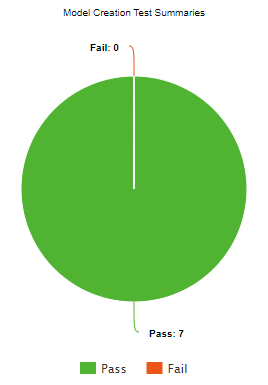
\includegraphics{./model_creation_pie_chart.png}
    \caption{Test data summary for the model creation tests.}
    \label{fig:creation_chart}
\end{figure}

\subsection{Specific Unit Tests}

Apart from the above common tests, some models require more specific tests for the custom methods the team created. This section will detail these extra tests. Some inputs will be in plain text, while others will use plain language for better descriptions.

\begin{longtable}{|>{\raggedright\arraybackslash} p{.18\linewidth} |>{\raggedright\arraybackslash} p{.275\linewidth} |>{\raggedright\arraybackslash} p{.2\linewidth}|>{\raggedright\arraybackslash} p{.2\linewidth} |>{\centering\arraybackslash} p{.1\linewidth}|}
\caption{Specific Tests Description with Results}
\label{tab:funcTestResults}
\\ \hline \textbf{Description} & \textbf{Inputs} & \textbf{Expected Output} & \textbf{Actual Output} & \textbf{Result} \\
\hline
\endfirsthead

\multicolumn{5}{c}
{{\bfseries \tablename\ \thetable{} -- continued from previous page}} \\
\hline \multicolumn{1}{|c|}{\textbf{Description}} & \multicolumn{1}{c|}{\textbf{Inputs}} & \multicolumn{1}{c|}{\textbf{Expected Output}} & \multicolumn{1}{c|}{\textbf{Actual Output}} & \multicolumn{1}{c|}{\textbf{Result}} \\ \hline 
\endhead

\hline \multicolumn{5}{|r|}{{Continued on next page}} \\ \hline
\endfoot

\endlastfoot
Shop, Get Employees: Get the list of employees working for a shop. & \textit{Shop}: \texttt{{'shop\_owner': 'testuser'}, \textttt{'shop\_email': 'testemail@test.com'}, \texttt{'id': 0}}, \textit{Employee}: \texttt{'username': 'testemployee', 'shop': '0'} & \texttt{<QuerySet>} of \textit{Employee} & \texttt{<QuerySet>} of \textit{Employee} & \textcolor{Green}{Pass} \\
\hline
Shop, Has Employee: Check whether an employee is working at the shop. & \textit{Shop}: \texttt{('shop\_owner': 'testuser', 'shop\_email': 'testemail@test.com','id': 0)}, \textit{Employee}: \texttt{'username': 'testemployee', 'shop': '0', 'id': 0}, \textit{id}: \texttt{0} & True & True & \textcolor{Green}{Pass} \\
\hline
 Service, Update Service: Partially update an already created service with a new part. & Existing Service object, including one part as its part list. A new part distinct from the part already in the Service object is queried to replace the old part.& The same service object is returned with the same values, aside from the list of parts associated with the object, which should be updated to the new part. & The service object is returned with the correct new parts list. &  \textcolor{Green}{Pass} \\
\hline
Quote Request, Get Quote Request Status: Get the status of the quote request from the associated quote. & Quote Request object that has an associated Quote object where Quote.status = \texttt{'new\_quote'}. & Quote Request Status = Quote Status = \texttt{'new\_quote'} & QuoteRequest. status = \texttt{'new\_quote'} &  \textcolor{Green}{Pass} \\
\hline
\end{longtable}

\section{Changes Due to Testing}

After concluding testing and receiving feedback from the usability survey, a number of changes and upgrades have been considered for the next revision of the project. For the functional tests, three tests failed due to missing features needed to achieve functional requirements. The features, which include shop owner account details/edit page, employee deletion, and search bars for all list pages, will be added in the next development stage of the application. All functional tests will be re run to ensure proper integration of the features. 

Furthermore, taking feedback from our surveyed focus group, we will be improving how navigation works throughout our application to enhance usability. We will also confirm all pages have uniformity in fonts, spacing and elements to improve visual appeal. Lastly we will be implementing a feature to enable customers and shop owners to comment on quotes and quote requests based on feedback given at the Rev0 demo.

\section{Automated Testing}

A limited number of front-end component-wise unit tests were written using Jest, a library for testing React components. Smoke tests were written for key components. These tests would check that each components renders correctly, and with the correct styles. These tests were then set to run on each commit using GitHub actions.

\section{Non-Dynamic Testing}

As specified in the VnV Plan, the team undertook different types of non-dynamic testing to verify and validate the application. This section will detail the results.

\subsection{Code Review}

Upon attempting to push code into the main branch of the GitHub repo, a code review was performed. Code required at least 1 member of the team to review and approve it in order to be implemented. The member who wrote the code would, if required, provide information about what was implemented and how to test it, and the member reviewing the code was allowed to suggest changes.

\subsection{Document Review}

Document reviews were carried out as each document was completed. If applicable, related documents were also reviewed. Document reviews consisted of the team reviewing documentation in order to determine if it met the current status of the project. If the document was not up to standards, it was updated accordingly.
\\\\
\noindent
At the current moment in time, a final documentation review has not been done, however, before the completion of the project, each document will be reviewed separately.

\subsection{Walkthroughs}

Informal walkthroughs were performed to generate test cases for the Verification and Validation Plan. Team members paired up with one other member to inspect parts of the code and generate test cases. Through this method test cases, along with various inputs for the given test cases were thought up and written into the Verification and Validation Plan, and eventually implemented into the code base to be run using continuous integration.

\section{Further Results}

This section will cover any further verification or validation that was carried out as part of the project.

\section{SRS Verification}

As listed in the Verification and Validation plan, requirements described in the SRS were validated. Requirements were evaluated and modified in order to meet the specified criteria.

\section{Design Verification}

The design of the project was created using Figma, as described in the project's design documents. Verification was carried out by consulting our Supervisor, Nabil Ibrahim. According to Mr. Ibrahim's comments, the design was modified and updated to meet his needs.

\section{Automated Tools}

As specified in the Verification and Validation plan, automated testing tools were used to facilitate easier development on the project's code-base through the use of GitHub Actions.

\section{Trace to Requirements}

\begin{table}[H]
  \centering
  \caption{Traceability Table for Functional Test Cases and Requirements}
  \label{tab:FRTraceReq}

 \makebox[\textwidth]{\begin{tabular}{|c|c|} 
    \hline
     \textbf{Test Case ID} & \textbf{Related Requirement(s)}\\ 
    \hline 
    \hline
    FT-RT-1 & FR-1\\
    \hline
    FT-RT-2 & FR-2\\
    \hline
    FT-RT-3 & FR-3\\
    \hline
    FT-RT-4 & FR-4\\
    \hline
    FT-RT-5 & FR-6\\
    \hline
    FT-RT-5.1 & FR-6\\
    \hline
    FT-RT-6 & FR-7\\
    \hline
    FT-RT-7 & FR-5, FR-13, FR-14\\
    \hline
    FT-RT-7.1 & FR-5, FR-13, FR-14\\
    \hline
    FT-RT-8 & FR-8\\
    \hline
    FT-RT-9 & FR-29\\
    \hline
\end{tabular}
\quad
  \begin{tabular}{|c|c|} 
    \hline
     \textbf{Test Case ID} & \textbf{Related Requirement(s)}\\ 
    \hline 
    \hline 
    FT-RT-9.1 & FR-33\\
    \hline
    FT-RT-10 & FR-10, FR-11, FR-22\\
    \hline
    FT-RT-10.1 &  FR-11, FR-32\\
    \hline
    FT-RT-10.2 & FR-11, FR-32\\
    \hline
    FT-RT-11 & FR-16\\
    \hline
     FT-RT-11.1 & FR-16\\
    \hline
     FT-RT-11.2 & FR-16\\
    \hline
    FT-RT-12 & FR-22\\
    \hline
    FT-RT-13 & FR-23\\
    \hline
    FT-RT-14 & FR-17\\
    \hline 
    FT-RT-15 & FR-24\\
    \hline
\end{tabular}}
\end{table}

\begin{table}[H]
  \centering
  \caption{Traceability Table for Non-Functional Test Cases and Requirements}
  \label{tab:NFRTraceReq}
 \makebox[\textwidth]{\begin{tabular}{|c|c|} 
    \hline
     \textbf{Test Case ID} & \textbf{Related Requirement(s)}\\ 
    \hline 
    \hline
    NFT-LF-1 & NFR-1\\
    \hline
    NFT-LF-2 & NFR-4\\
    \hline
    NFT-UT-1 & NFR-6, NFR-7\\
    \hline
    NFT-UT-2 & NFR-10\\
    \hline
    NFT-PF-2 & NFR-12\\
    \hline
\end{tabular}}
\end{table}
		
\section{Trace to Modules}		

The following tables illustrates the traceability between functional  tests and the modules described in our \href{https://github.com/HKanwal/kapstone/blob/main/docs/Design/MG/MG.pdf}{Module Guide}.

\begin{table}[H]
  \centering
  \caption{Traceability Table for Functional Test Cases and Modules}
  \label{tab:FRTraceMod}

 \makebox[\textwidth]{\begin{tabular}{|c|c|} 
    \hline
     \textbf{Test Case ID} & \textbf{Related Module(s)}\\ 
    \hline 
    \hline
    FT-RT-1 & M1, M2, M8\\
    \hline
    FT-RT-2 & M1, M2, M4\\
    \hline
    FT-RT-3 & M1, M2, M8\\
    \hline
    FT-RT-4 & M1, M2, M8\\
    \hline
    FT-RT-5 & M1, M8\\
    \hline
     FT-RT-5.1 & M1, M8\\
    \hline
    FT-RT-6 & M1, M8\\
    \hline
    FT-RT-7 & M1, M3\\
    \hline
    FT-RT-7.1 & M1, M3\\
    \hline
    FT-RT-8 & M1, M2\\
    \hline
    FT-RT-9 & M1, M5\\
    \hline
\end{tabular}
\quad
  \begin{tabular}{|c|c|} 
    \hline
     \textbf{Test Case ID} & \textbf{Related Module(s)}\\ 
    \hline 
    \hline 
    FT-RT-9.1 & M1, M5\\
    \hline
    FT-RT-10 & M1, M5, M6\\
    \hline
    FT-RT-10.1 & M1, M5, M6\\
    \hline
    FT-RT-10.2 & M1, M5, M6\\
    \hline
    FT-RT-11 & M1, M9\\
    \hline
    FT-RT-11.1 & M1, M9\\
    \hline
    FT-RT-11.2 & M1, M9\\
    \hline
    FT-RT-12 & M1, M3, M6\\
    \hline
    FT-RT-13 & M1, M9\\
    \hline
    FT-RT-14 & M1, M3, M8\\
    \hline 
    FT-RT-15 & M1, M7\\
    \hline
\end{tabular}}
\end{table}


\bibliographystyle{plainnat}
\bibliography{../../refs/References}

\newpage{}
\section*{Appendix --- Reflection}

The information in this section will be used to evaluate the team members on the
graduate attribute of Reflection.  Please answer the following question:

\begin{enumerate}
  \item In what ways was the Verification and Validation (VnV) Plan different
  from the activities that were actually conducted for VnV?  If there were
  differences, what changes required the modification in the plan?  Why did
  these changes occur?  Would you be able to anticipate these changes in future
  projects?  If there weren't any differences, how was your team able to clearly
  predict a feasible amount of effort and the right tasks needed to build the
  evidence that demonstrates the required quality?  (It is expected that most
  teams will have had to deviate from their original VnV Plan.)
\end{enumerate}
\\
The Verification and Validation Plan differed mostly in the content of the tests that were actually implemented into the code-base. Tests were added and removed from the VnV Plan in order to match the ones decribed in the VnV Report. These changes occurred because our requirements have changed since the beginning of the project, and our implementation, now almost finalized, differs from the vision created by Revision 0 of our SRS. In the future, now that the team has experience building something of this scale, we may be able to anticipate the requirements of a project more accurately to its final design. If the requirements are more accurate, this increases the accuracy of the mapping of the VnV Plan to what was actually implemented, therefore making the VnV Report have fewer changes.

\newpage{}
\section*{Appendix --- Usability Survey Results}
\label{sec:AppSurveyResults}
The following figures are charts gathered by Google Forms depicting our usability survey results. For each question, a rating was provided on a scale of 1 to 5 (where 1 represents a poor review and 5 represents a strong review).
\begin{figure}[!h]
    \centering
    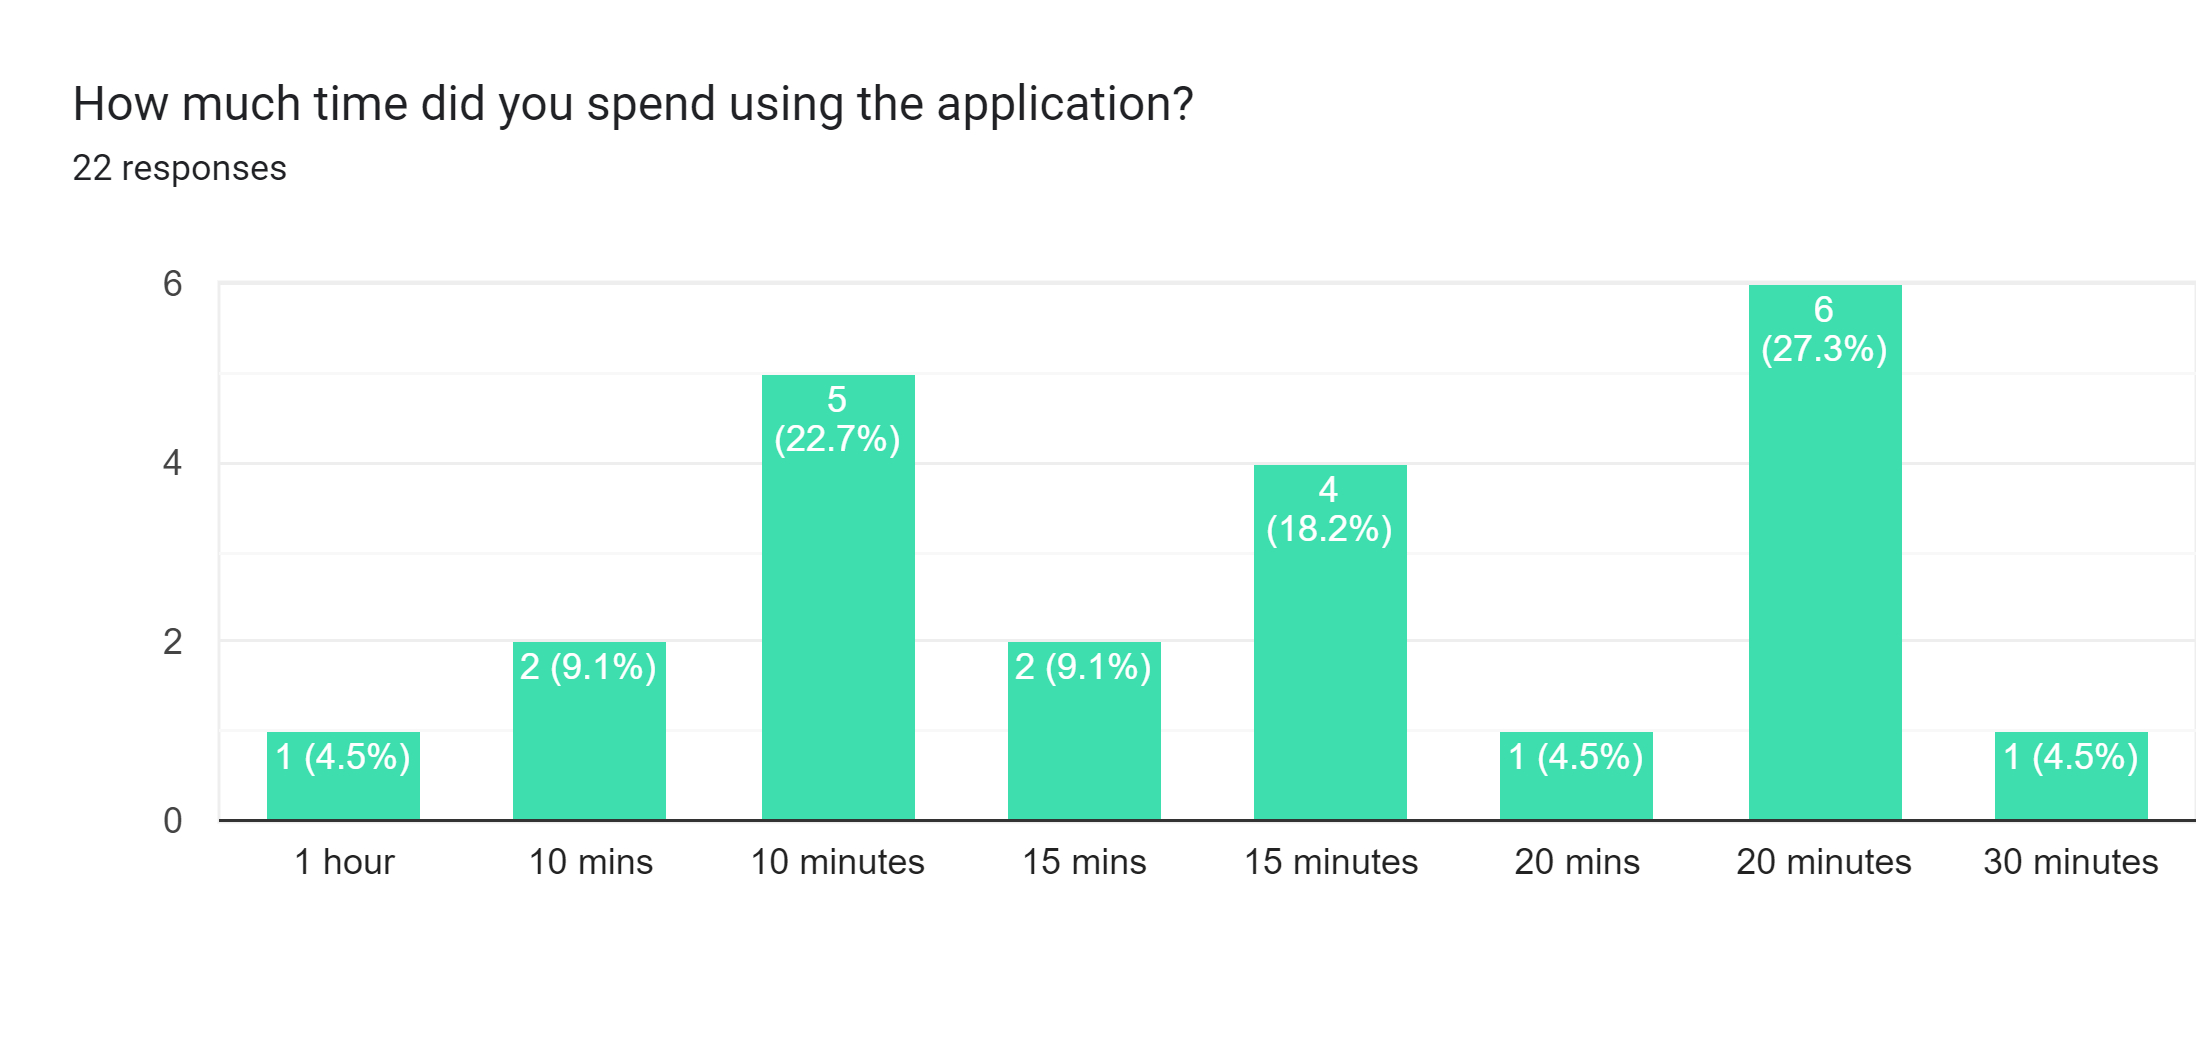
\includegraphics[width=\textwidth]{time_spent.jpg}
    \caption{Survey Result - Time Spent on the App}
    \label{fig:time_spent}
\end{figure}
\begin{figure}[!h]
    \centering
    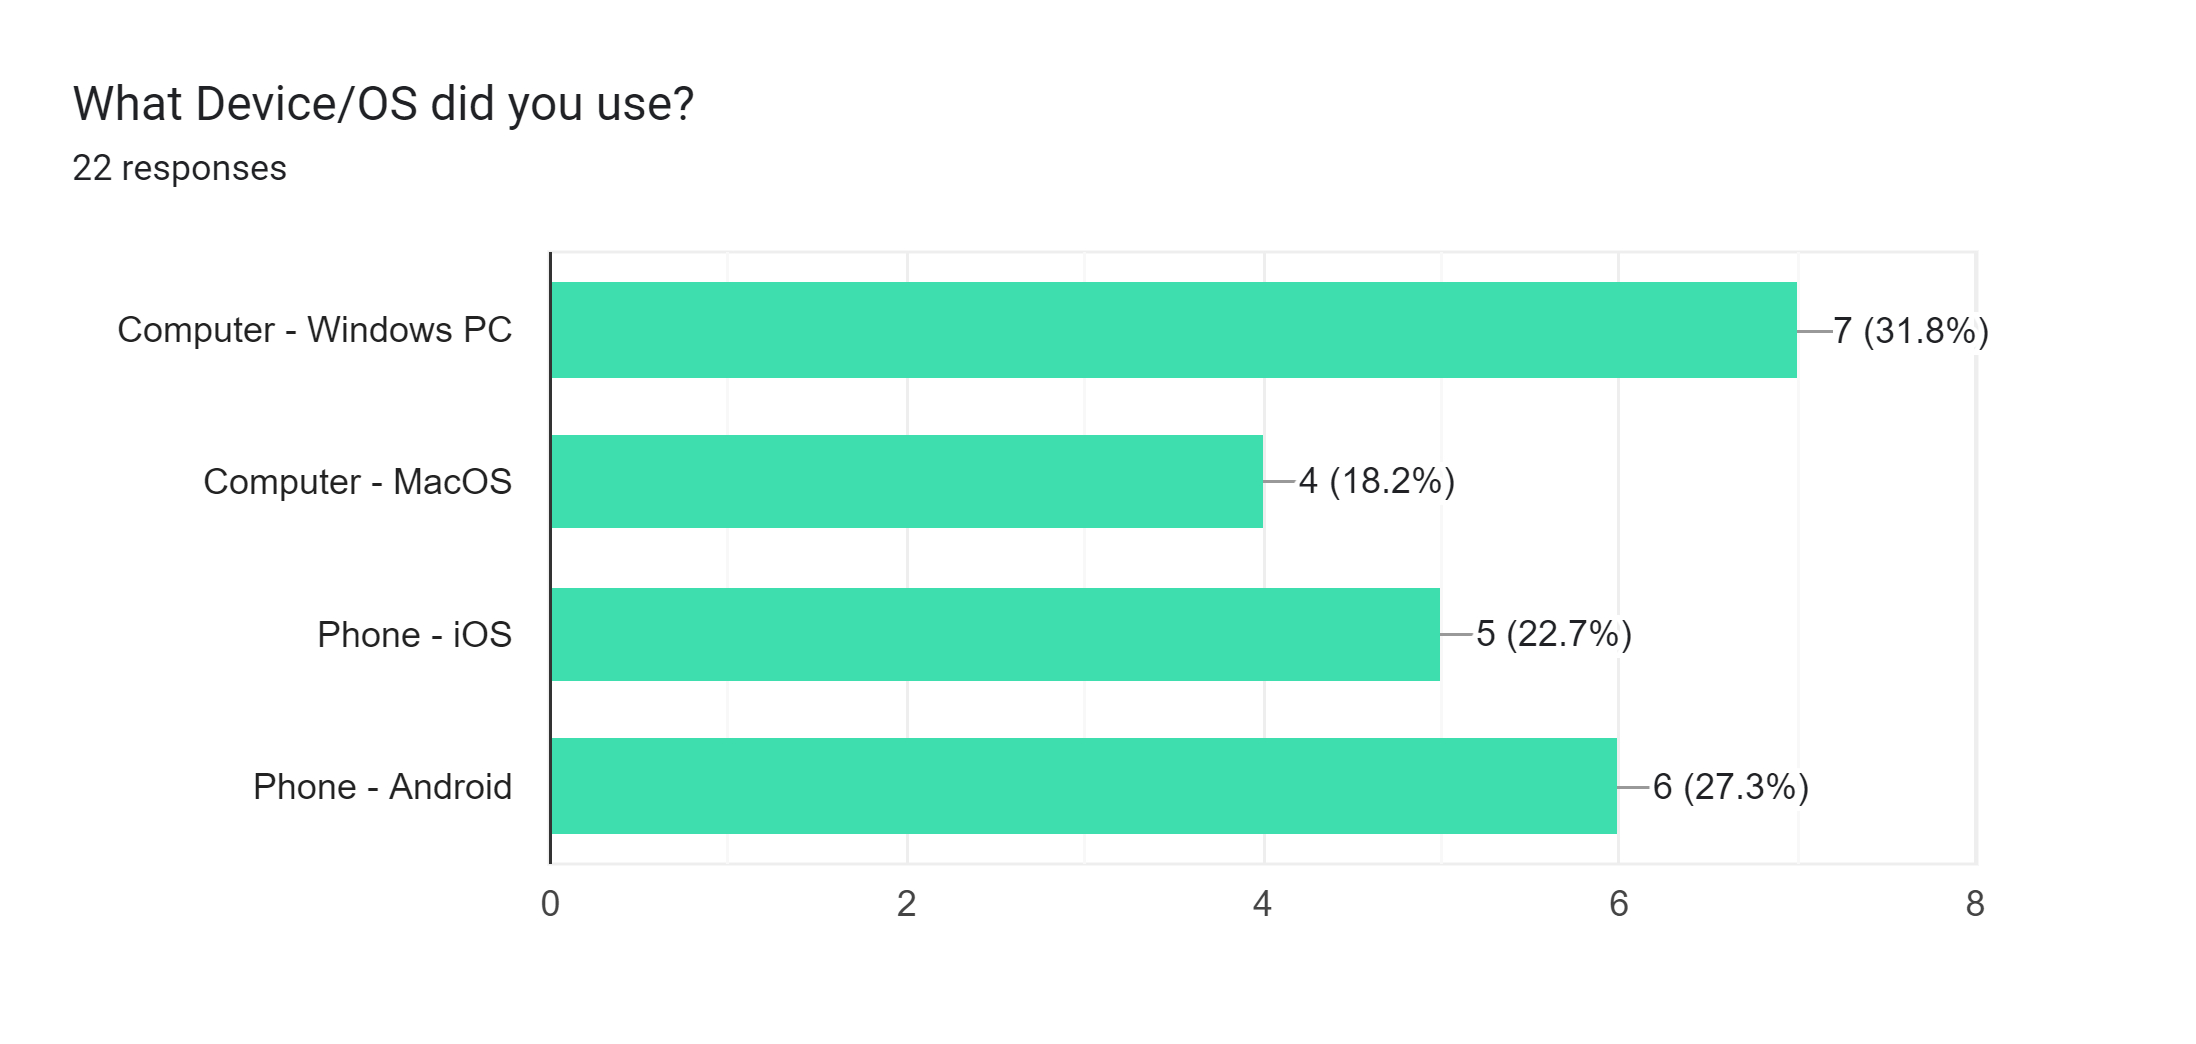
\includegraphics[width=\textwidth]{device_used.jpg}
    \caption{Survey Result - Device Used}
    \label{fig:device_used}
\end{figure}
\begin{figure}[!h]
    \centering
    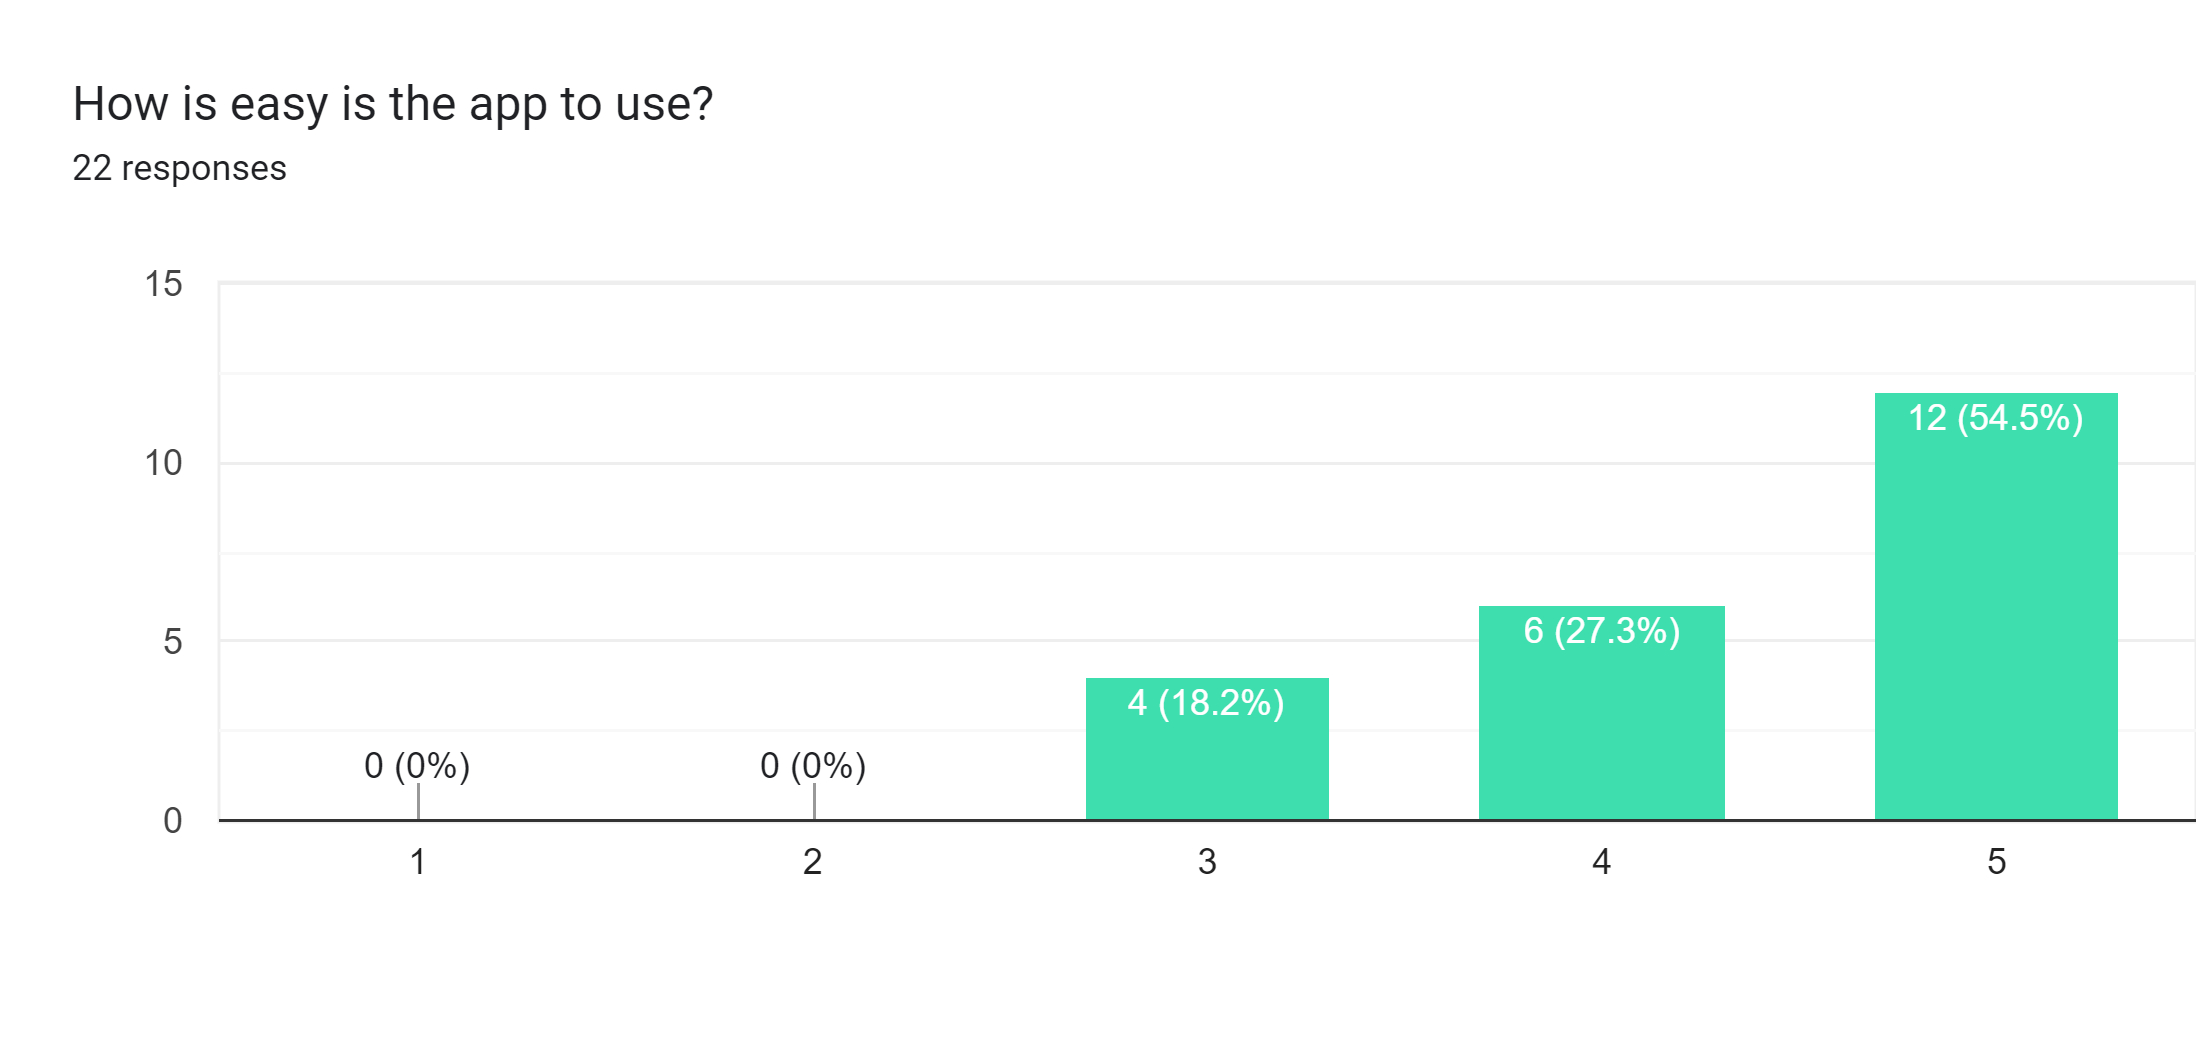
\includegraphics[width=\textwidth]{ease_of_use.jpg}
    \caption{Survey Result - Ease of Use}
    \label{fig:ease_of_use}
\end{figure}
\begin{figure}[!h]
    \centering
    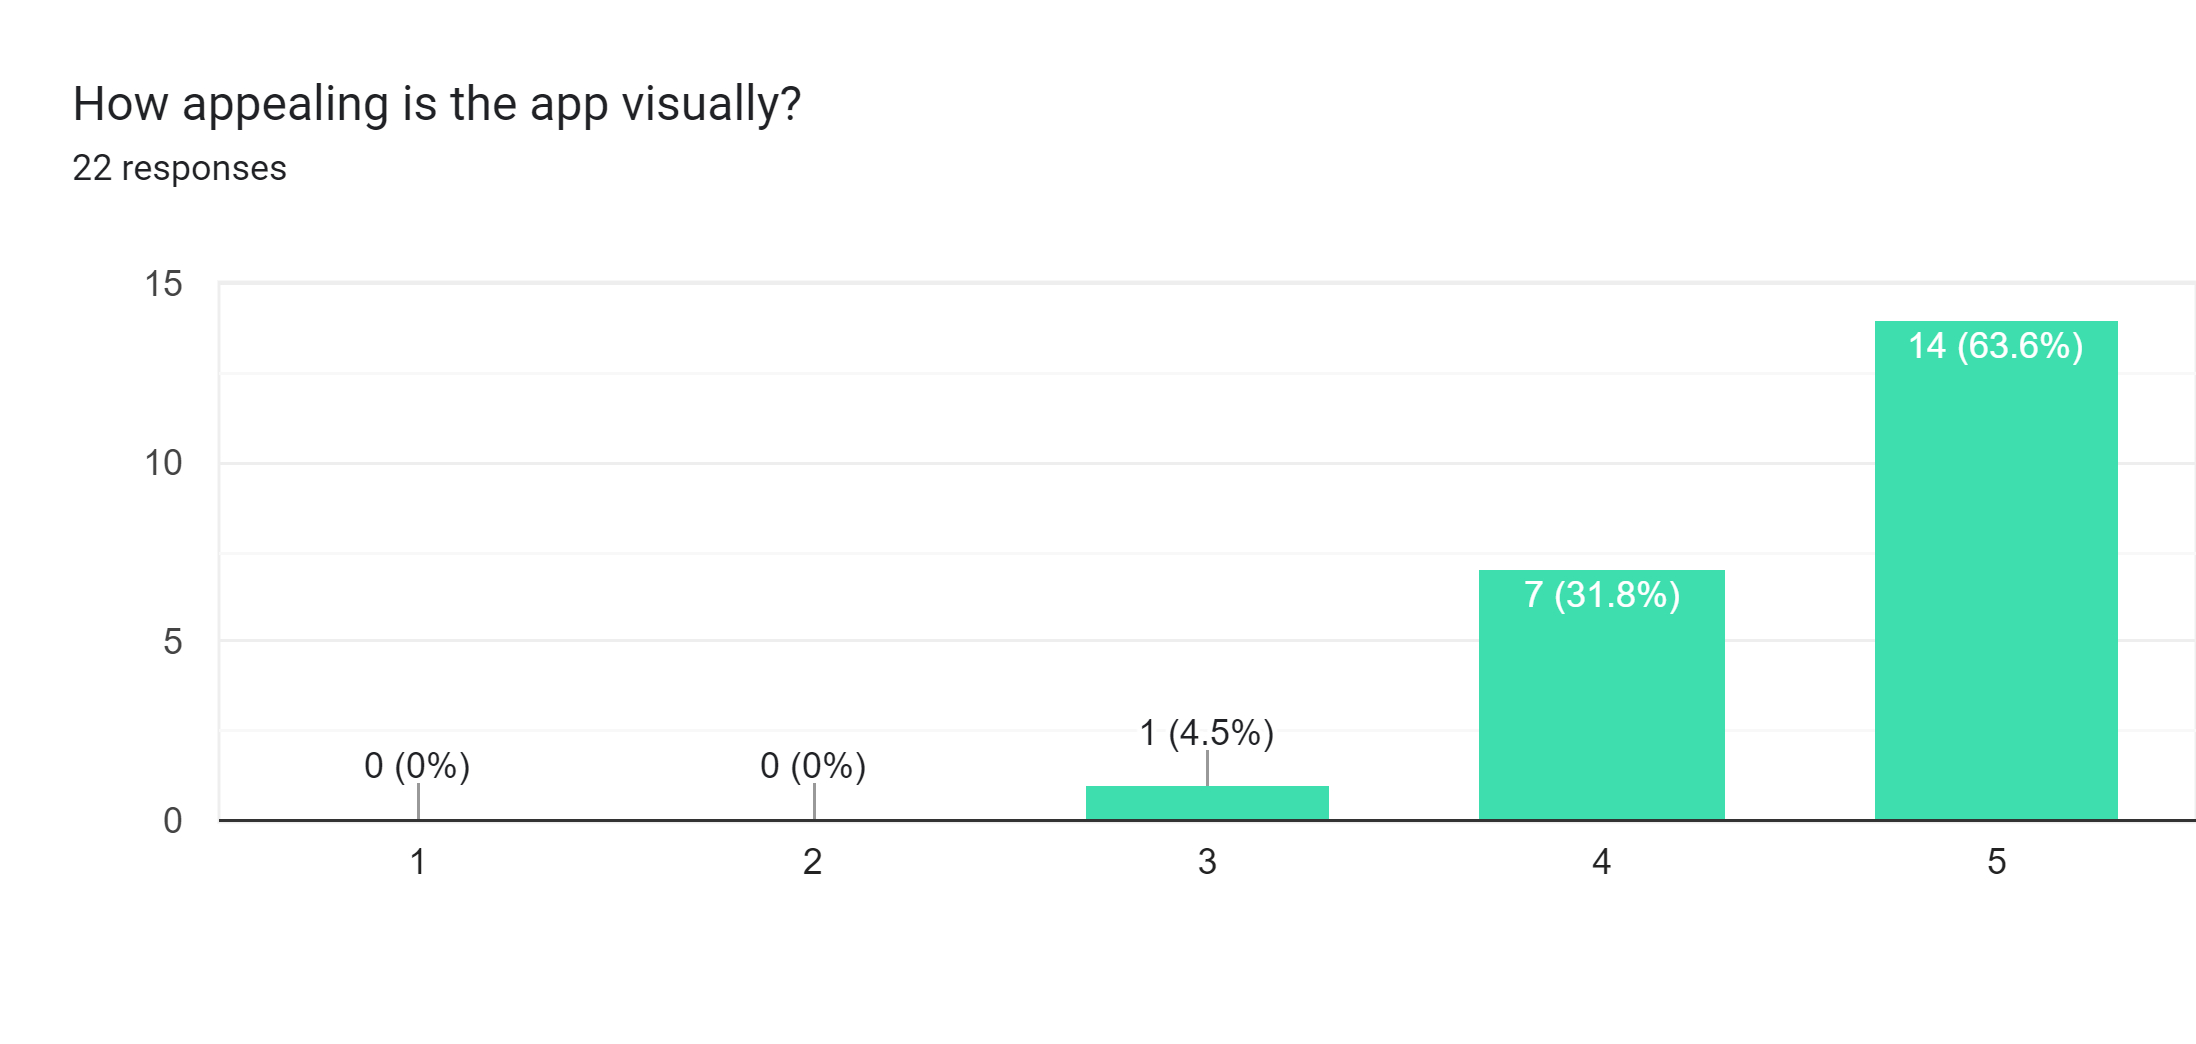
\includegraphics[width=\textwidth]{visual_appeal.jpg}
    \caption{Survey Result - Visual Appeal}
    \label{fig:visual_appeal}
\end{figure}
\begin{figure}[!h]
    \centering
    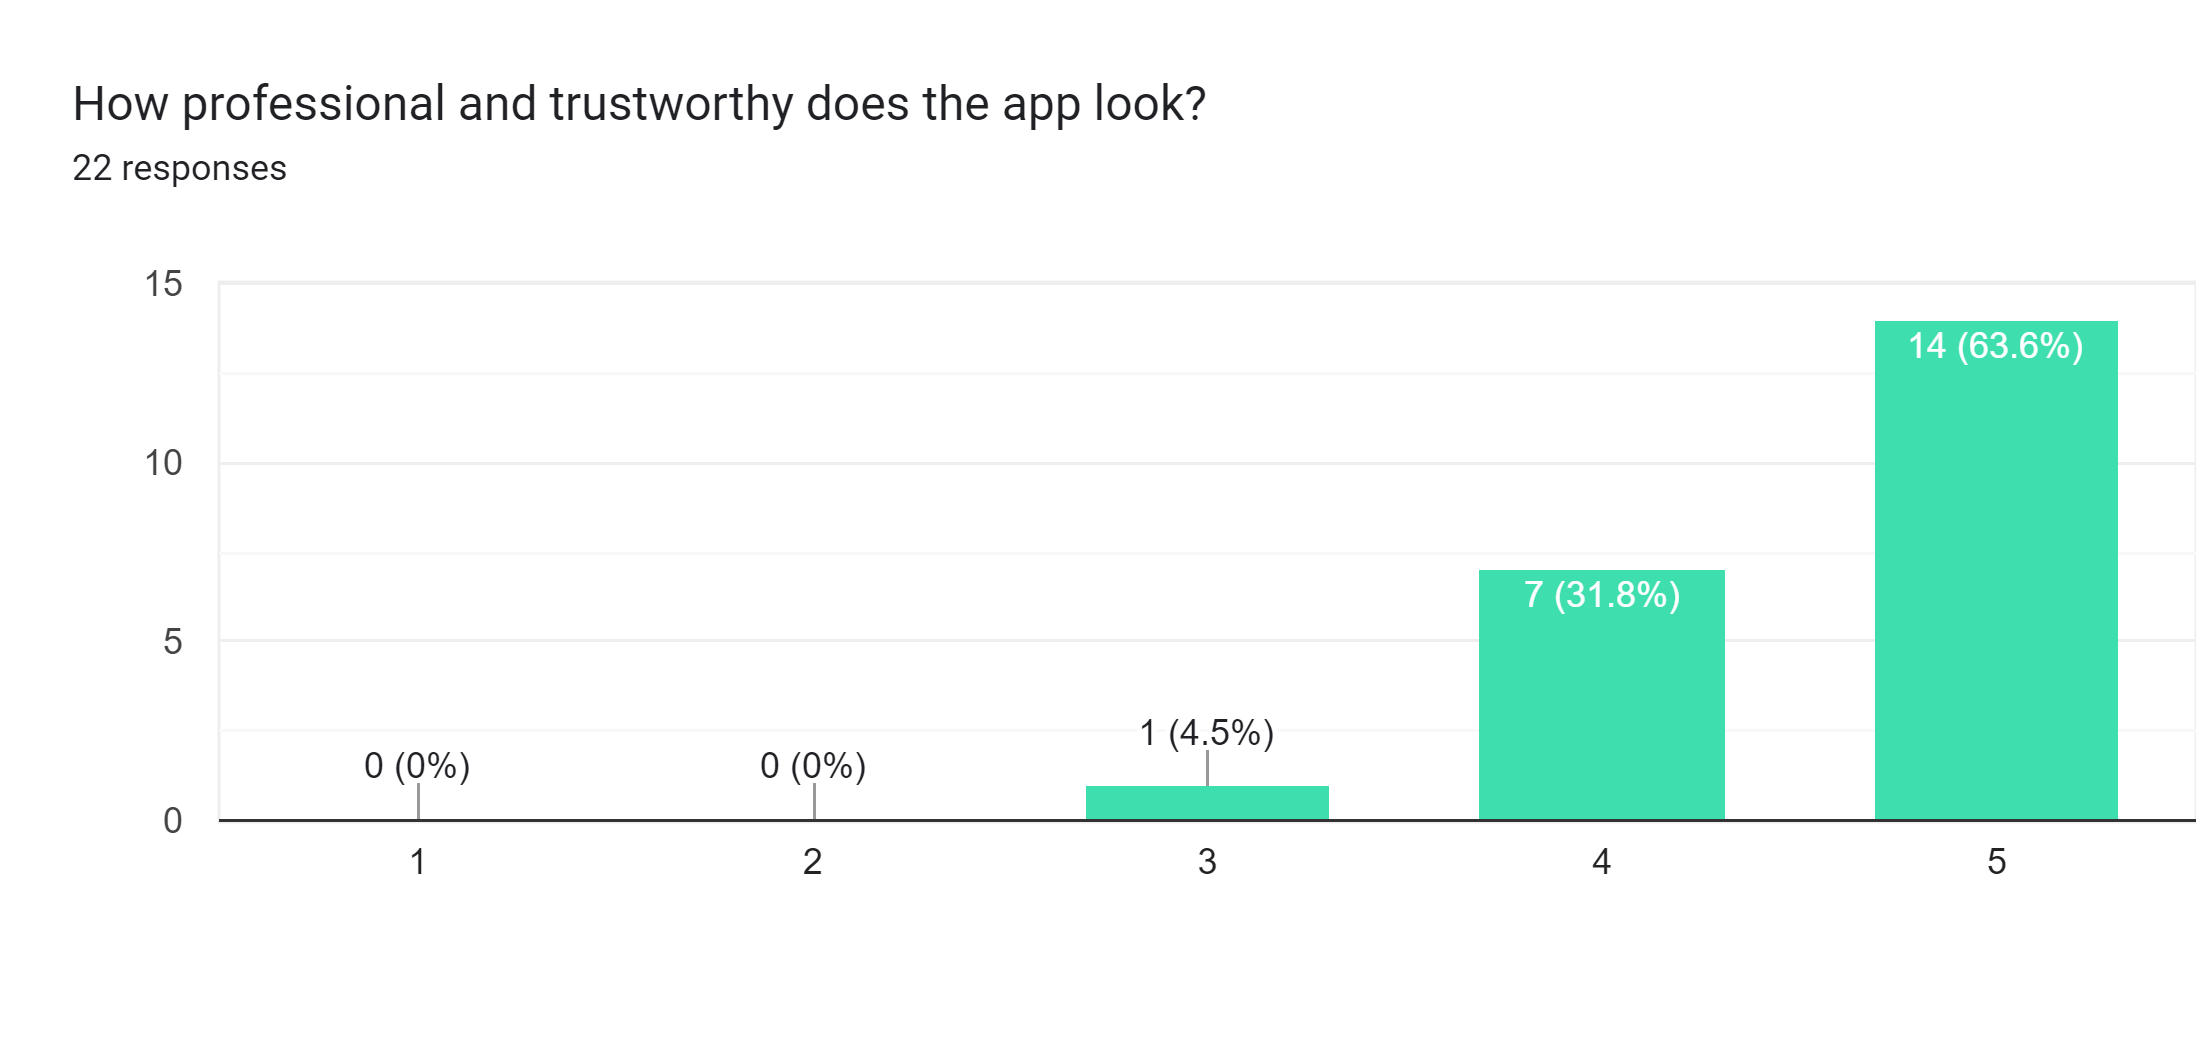
\includegraphics[width=\textwidth]{professionalism.jpg}
    \caption{Survey Result - Professionalism and Trustworthiness}
    \label{fig:professionalism}
\end{figure}
\begin{figure}[!h]
    \centering
    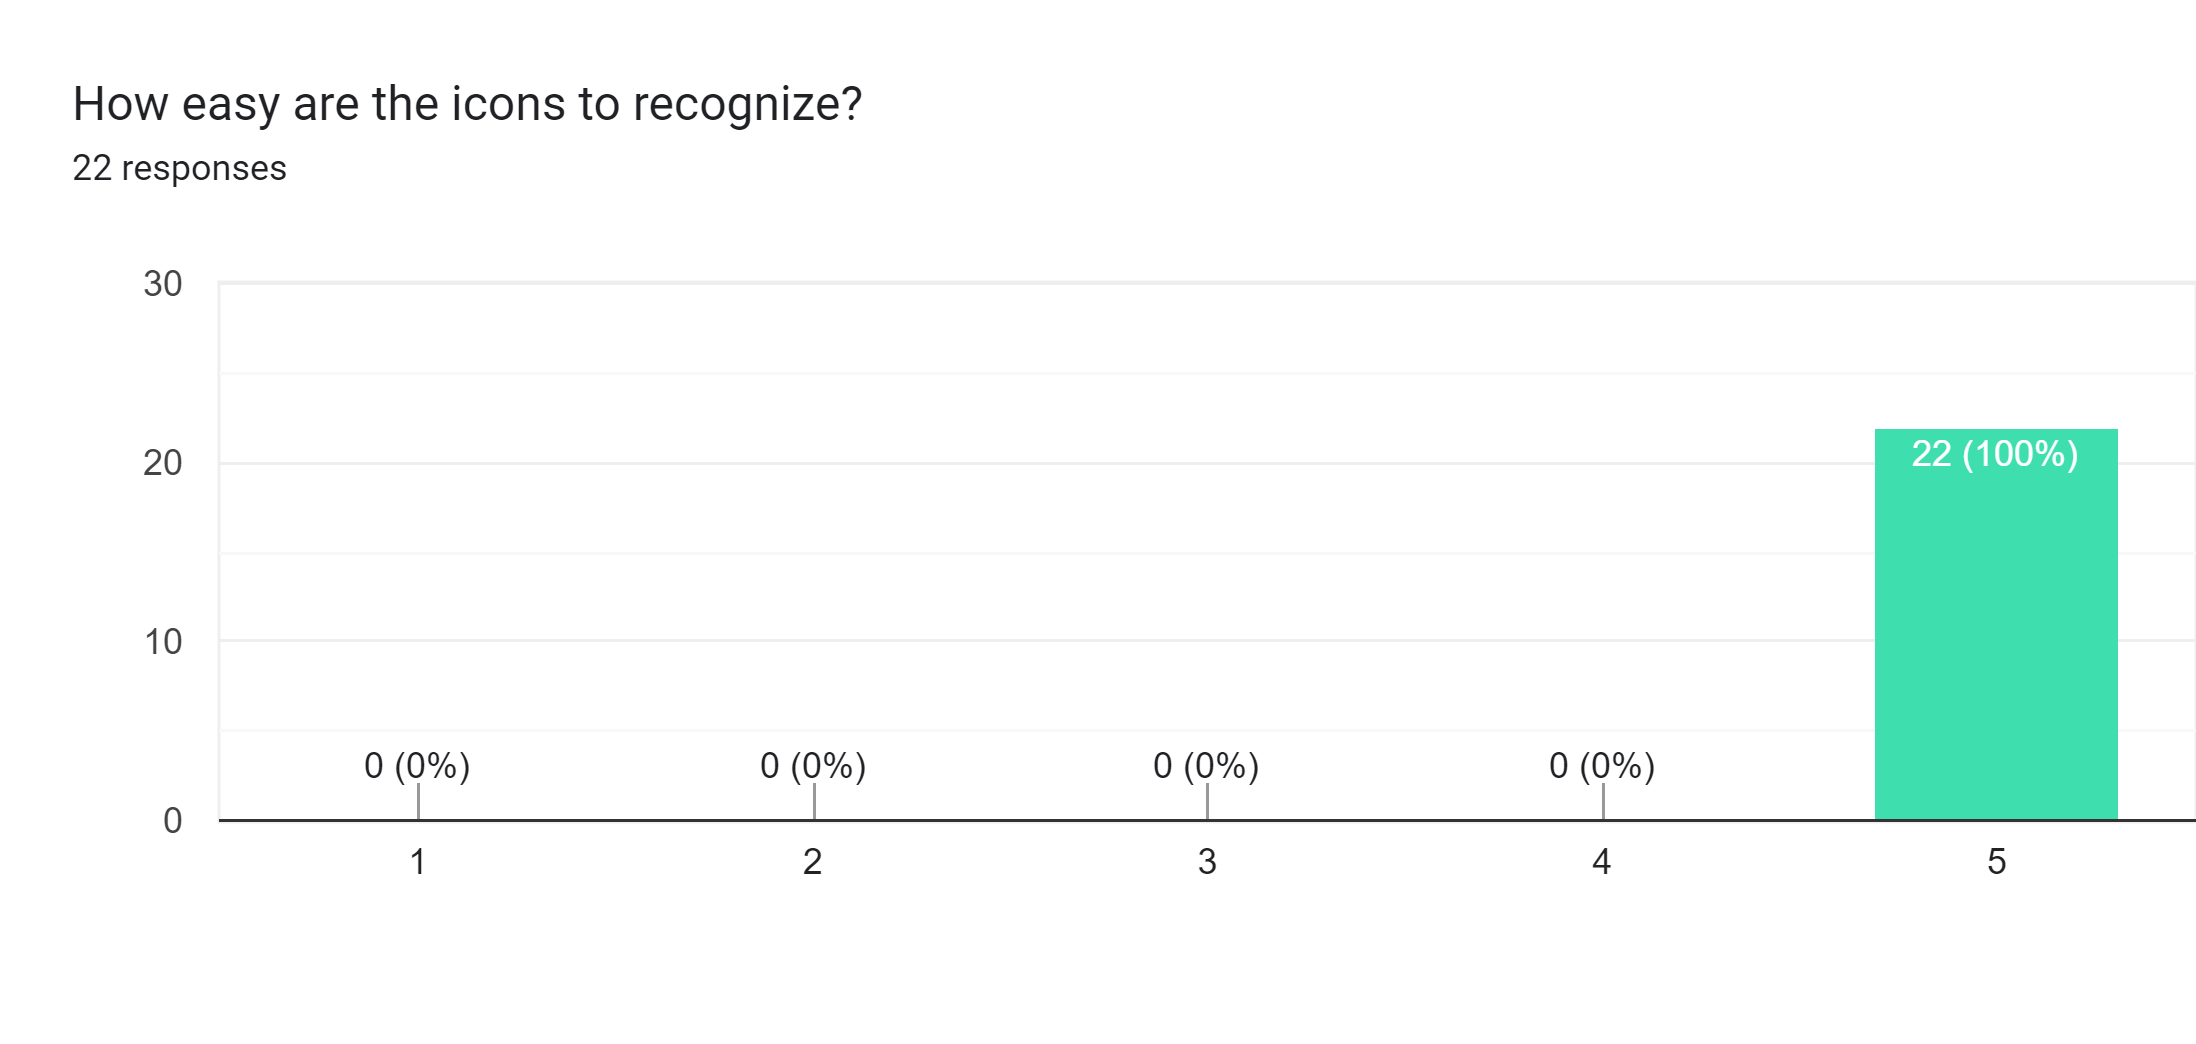
\includegraphics[width=\textwidth]{recognize_icons.jpg}
    \caption{Survey Result - Recognizable Icons}
    \label{fig:recognize_icons}
\end{figure}


\end{document}